\chapter{State of the art}

\section{Ray Tracing}

\par
Ray tracing one frame can be, simultaneously, a computationally demanding task and an embarrassingly parallel task.
As tracing rays is a recursive process which aims to calculate the luminance of light of each individual pixel separately.
At least one ray is shot per pixel and in a naive approach each ray would be intersected with all the objects in the scene in order to determine which one is the closest primitive intersecting that given ray.
To evaluate the light intensity that an object scatters towards the eye, the intensity of the light reaching that object has to be evaluated as well.
Ray tracing achieves this by shooting additional secondary rays, because when a ray hits a reflecting or transparent surface, one or more secondary rays are cast from that point, simulating the reflection and refraction effects.

\begin{figure}[H]
	\centering
	\caption{Illustration of a typical ray tracer algorithm.}
	\label{Illustration of a typical ray tracer algorithm.}
	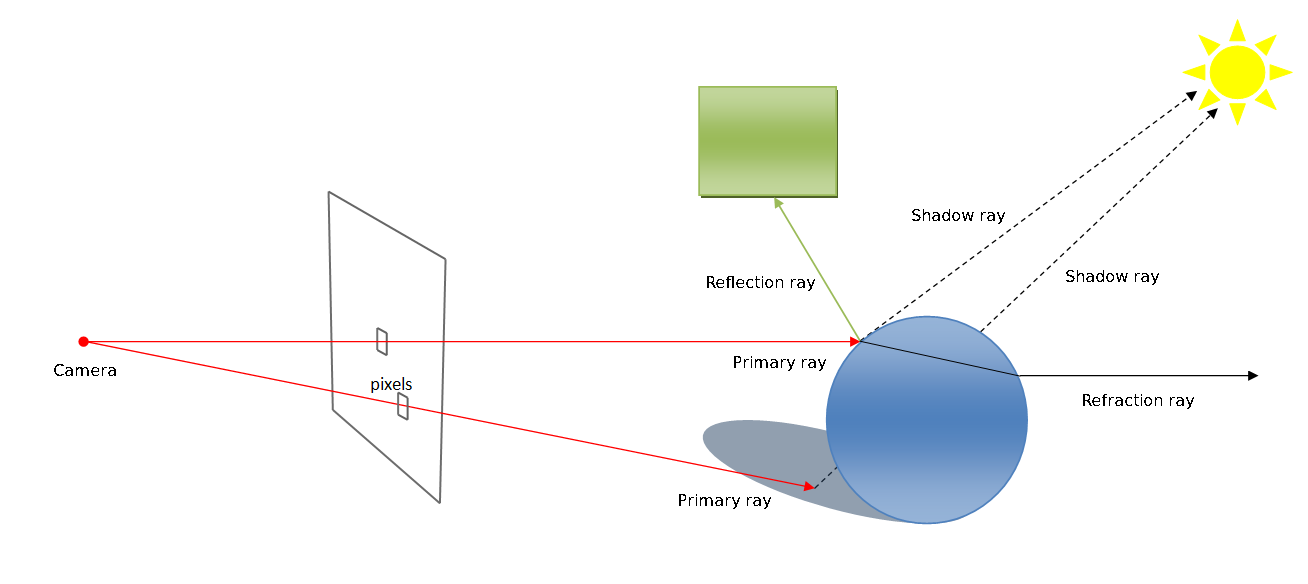
\includegraphics[keepaspectratio,scale=0.3]{Ray_Tracing.png}
\end{figure}

\par
A typical image of 1024 x 1024 pixels tends to cast at least a million primary rays and a multiple of that as shadow, reflection, refraction and secondary rays.
This is why ray tracing can't provide interactive frame rates with ease.

\section{Typical CPU features}

\par
Fortunately, the present state of available technology provides affordable machines with multiple CPU cores that can work in parallel and with great performance.
This is achieved thanks to features developed inside the processor like the cache, the multilevel pipeline, the hardware prefetching and SIMD instruction set already available in the current processors.

\par
The cache is a very small and fast multilevel memory inside the processor that temporarily stores the data read from the main memory.
This memory allows reading its content at a very low latency in the order of magnitude of around 1 nanosecond in the first level, 10 nanoseconds at second level and 50 nanoseconds at third level compared to the typical 100 nanoseconds of a DDR main memory.
The downside is that it is very small because its cost are much higher than a typical RAM memory.
Nowadays, the level 1 has 64kB, the level 2 has 256kB and the level 3 has 8 MB which is very little compared to the typical 16GB provided by the memory RAM.

\begin{figure}[H]
	\centering
	\caption{Illustration of a typical cache memory inside a microprocessor (\cite{CPU_Cache}).}
	\label{Cache.}
	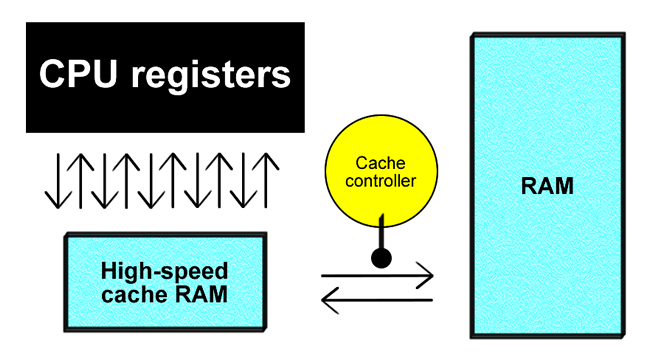
\includegraphics[keepaspectratio,scale=0.3]{cache.png}
\end{figure}

\par
The multilevel pipeline is another feature inside a processor which allows to reduce the processor's own latency by allowing a form of parallelism called instruction-level parallelism within a single processor.
Basically, one instruction is divided in some stages and it allows the possibility to execute different stages of different instructions simultaneously.
In the early days, the Classic RISC pipeline were typically divided in 5 stages:
\begin{itemize}  
	\item Fetching the instruction
	\item Decoding the instruction
	\item Executing the instruction where the arguments can be fetched from registers (1 cycle latency) or from memory (2 cycle latency)
	\item Memory access where it ensured that writing in memory was always performed in the same stage and allowed to use that value in another instruction before it was written in memory
	\item Writing back the value in the register
\end{itemize}
Nowadays, the current microprocessors have a pipeline with 8-14 stages and can be more complex than the Classic RISC, but the operating principle is the same.
This allows faster CPU throughput, which means the number of instructions that can be executed in a unit of time is greater, than it would otherwise be possible at a given clock rate.

\begin{figure}[H]
	\centering
	\caption{Illustration of the Classic RISC multilevel CPU pipeline (\cite{CPU_Pipeline}).}
	\label{Pipeline.}
	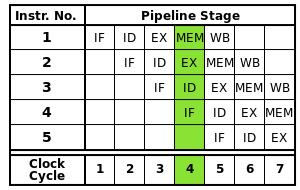
\includegraphics[keepaspectratio,scale=0.5]{Pipeline.png}
\end{figure}

\par
The hardware prefetching is, as the name implies, a feature in the processor that makes the processor fetch the data and the instructions before it really needs to execute.
This allows to reduce the time that the processor waits for the data in the main memory.

\par
Finally, SIMD instruction set is a set of special instructions that allows the processor to read or write bigger sizes of data.
Typically, a 64 bit processor can only work with 64 bits of information at a time during the execution of an instruction.
This feature can allow to read or write up to 512 bits by using special registers and additional ALUs provided in the processor.

\begin{figure}[H]
	\centering
	\caption{Illustration of a typical execution of SIMD extension (\cite{CPU_SIMD}).}
	\label{SIMD.}
	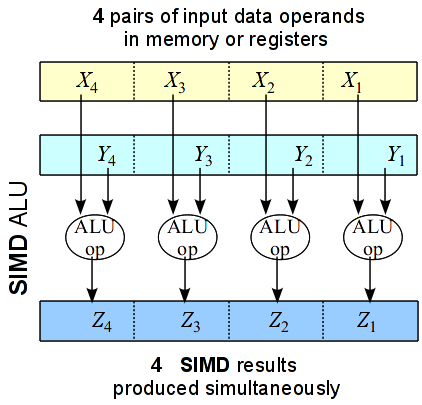
\includegraphics[keepaspectratio,scale=0.5]{SIMD.png}
\end{figure}

\par
Nowadays, even mobile devices like smart phones and tablets have multiple CPU cores with features similar to those described above.
This opens the possibility to execute more computationally demanding algorithms, like ray tracing, in these devices.

\section{Key features of Ray Tracing for this work}

\par
Ray tracing is an algorithm that can have a panoply of features or optimizations in order to reduce the time required to trace all the rays and / or to show the results as fast as possible.
It also, like any application, can have different types of software licenses and be executed in different platforms.

\par
For this work, the most important features in a ray tracer are: the type of software license, the platform where can be executed, interactivity, progressive and the type of rendering components.

\subsection{Type of software license}

\par
A software application can have different type of software license, but in order to simplify this dissertation, the software license were grouped into 3 types: Free, Commercial and Open Source.
The license Free means that the user has the right to execute freely the application but cannot copy, modify or distribute the implemented code.
The license Commercial means that the user cannot even execute the application without buying it first and cannot copy, modify or distribute the implemented code.
The license Open Source means that the user has the right to execute freely the application and can even copy, modify and distribute the implemented code.
The software license is very important in this work because it lets the user know if he can develop something over the provided software or if he can just use the application.

\subsection{Platform}

\par
An application can only be executed in the platforms that the developers compiled the code for.
So, a ray tracer that can be executed in a desktop may also or may not be executed on another platform, like a mobile device.
This information is very important in this work because it inform us whether a ray tracer can be executed in a mobile device with the typical Operating System like Android, iOS or Windows 10 Mobile.

\subsection{Interactivity}

\par
In ray tracing, interactivity means rendering an image with a very low response time, like a few milliseconds per frame.
An interactive ray tracer can render a scene with multiple frames per second.

\subsection{Progressive}

\par
A typical ray tracer shows the rendered image only after the whole process is complete.
A progressive ray tracer is a ray tracer that updates the color of pixels in the screen as soon as the rays are traced, instead of waiting for the rendering process to complete.
This means that an image is rendered quickly with some aliasing or noise and it is progressively improved over time.

\subsection{Types of Rendering Components}

\par
A ray tracer can be developed with the different rendering components programmed separately.
Some examples of rendering components are: Integrators, Cameras, Scenes, Samplers, Shapes, Lights and Accelerator Structures.
In some ray tracers, these rendering components can even be programmable by the user.
This is very important because it allows the user to develop his own renderer based in ray tracing without having to develop every feature in the ray tracer.

\section{Related work}

\par
The possibility of rendering an image with ray tracing was demonstrated in 1980 by Whitted (\cite {Whitted}) and since then the number of libraries that provide basic ray tracing functionalities increased greatly.
There is a wide range of different ray tracers available today for the programmer to use, yet the majority can only be used with the traditional personal computer hardware (desktop or laptop).

\par
The table \ref{comparison state of the art} shows some applications or frameworks that use ray tracing available today and compares them according to their type of license, platform compatibility, interactivity, progressive and whether they allow development of your own rendering components like the integrator and sampler.
Note that some of these ray tracers provide only the engine with the basic ray tracing functions, such as creating rays and intersecting them with geometric primitives, so the rendering components are only programmable if the application that uses the engine supports it.
During the research of the available ray tracers, others than the ones presented in the table were found, but they were excluded because the documentation was very poor without explaining the basic functionalities provided or because there was no documentation at all.

\begin{table}[H]
\centering
\caption{Comparison of different applications/frameworks that use ray tracing}
\label{comparison state of the art}
\hspace*{-2.0cm}
\scriptsize
\begin{tabular}{|c|c|c|c|c|c|c|c|}
\hline
\textbf{Product}											& \textbf{License}	& \textbf{Platform}	& \textbf{Mobile}		& \textbf{Interactivity}	& \textbf{Progressive}	& \makecell{\textbf{Programmable} \\ \textbf{Components}}\\ \hline
Optix (\cite{Optix})											& F                	& Nvidia GPU 			& N				& Y                  	& Y                 		& Y\\ \hline
Optix Prime (\cite{OptixPrime})								& F                	& CPU \& Nvidia GPU 	& N				& Y                  	& Y                 		& Y\\ \hline
RenderMan RIS (\cite{RIS})									& C       	& CPU 		             & N                  		& Y                 		& Y				& Y\\ \hline
OctaneRender (\cite{OctaneRender})							& C       	& GPU 		             & N                  		& Y                 		& Y				& N\\ \hline
Embree (\cite{Embree}										& O     	& Intel CPU			& N				& Y                  	& Y                      	& Y\\ \hline
Radeon Rays (\cite{RadeonRays})							& O	& CPU \& GPU		& N				& Y                    	& Y                     	& Y\\ \hline
PBRT (\cite{PBRT})	 									& O	& CPU				& N                 		& N                 		& N				& N\\ \hline
Visionaray (\cite{Visionaray})									& O     	& CPU \& Nvidia GPU	& N                  		& Y				& Y                  	& N\\ \hline
YafaRay	(\cite{YafaRay})									& O     	& CPU 				& N                  		& N				& N                  		& N\\ \hline
tray\_rust (\cite{trayrust})									& O    	& CPU                  	& N                   	& N                  		& N                 		& N\\ \hline
micro-packet (\cite{micro-packet})							& O     	& Intel CPU 			& N                  		& N                  		& N 				& N\\ \hline
tray (\cite{tray})											& O     	& CPU 				& N				& N                     	& N                  		& N\\ \hline
The G3D Innovation Engine (\cite{G3D17})						& O	& CPU 				& N				& N                 		& N                 		& N\\ \hline
HRay (\cite{HRay})										& O     	& CPU                		& N                  		& N                      	& N				& N\\ \hline
Mitsuba (\cite{Mitsuba})										& O 	& CPU 				& N				& N                 		& N				& N\\ \hline
Indigo RT (\cite{IndigoRT})									& O 	& CPU \& GPU		& N				& Y                 		& N				& N\\ \hline
jsRayTracer (\cite{jsRayTracer})								& O 	& CPU 				& N				& Y                 		& Y				& N\\ \hline
Android CPU Raytracer (\cite{Android_CPU_Raytracer})			& O 	& CPU 				& Y (Android)		& Y                 		& N				& N\\ \hline
\end{tabular}
\normalsize
\end{table}

\subsection{Conclusions}

%Em que é que o que eu proponho é diferente das anteriores.

\par
As the table \ref{comparison state of the art} shows, there is a lack of generic ray tracing libraries for the mobile devices.
Although there are some closed-source ray tracing demo applications, only one ray tracer already available has some sort of documentation and is compatible with mobile devices, in this case with Android.
This ray tracer is open source, uses only the CPU of the device and has a good performance.
It even allows interactions with the objects during the render process.
But, it doesn’t support progressive rendering and also does not allow the programmers to use their own rendering components.

\par
This dissertation aims to fix this lack of libraries, by providing one that contains ray tracing basic functionalities and the ability to let the programmer be able to develop their own rendering components like the sampler, integrator, camera and shapes of virtual objects.
It also studies the drawbacks that these mobile devices may have comparing with the average multi-core personal computer hardware.
And finally, a small comparison was made with the Android CPU Raytracer (\cite{Android_CPU_Raytracer}) in order to illustrate the advantages and disadvantages of both.
This comparison is important because it enriches all the work done, as it demonstrates if the performance of the provided features are relatively efficient.